\section{Experiments}
\label{sec:expt}

\subsection{Evaluation data}

\paragraph{CoNLL} 
The CoNLL dataset ~\cite{Hoffart2011} contains 1,393 articles with
about 34K mentions, and the standard performance metric is
mention-averaged accuracy.  The documents are partitioned into train,
test-a and test-b.  Most authors report performance on the subset of
231 test-b documents with 4,483 linkable mentions.

\paragraph{TAC KBP} 
The TAC KBP datasets \cite{TAC2010,TAC2011,TAC2012} include 2,226 mentions
(2012) and 2,250 mentions (2011), of which roughly half are linkable
to the reference KB.  The competition evaluation includes $\NIL$
entities; participants are required to cluster $\NIL$ mentions across
documents so that all mentions of each unknown entity are assigned a
unique identifier.  For these datasets, we report in-KB accuracy,
overall accuracy (with all $\NIL$s in one cluster), and the competition
metric $B^{3+} F_1$ which evaluates $\NIL$ clustering.

\subsection{Experimental setup}

\subsubsection{Mention prior}

Our KB is derived from the Wikipedia subset of Freebase \todo{cite, download date?}, with about 4M entities. 
We use the KB to obtain a baseline prior over entities given a mention. As sources of alias counts, we use
Wikipedia page titles (including redirects and disambiguation pages), Freebase aliases, 
Wikipedia anchor text \todo{is this true -- we use wikilinks?},  and
\todo{CHECK} filtered anchor text from Web links into Wikipedia pages
\cite{singh12:wiki-links}.

As an optional additional source of aliases, we use the alias-entity mapping released
by \newcite{Hoffart2011}, obtained by extending the extending the
``means'' tables of YAGO \cite{hoffart2013yago2}. This mapping was released alonside
CoNLL gold entity annotations. When it was
published, it had 100\% mention recall on CoNLL, i.e. every annotated mention
could be mapped to at least one entity, and the set of entities included the gold entity. 
However, changes in canonical Wikipedia URLs, accented characters and
unicode usually result in mention losses over time, as not all URLs can be mapped to the KB.

For CoNLL only, we experiment with a third alias-entity mapping derived 
from \cite{Hoffart2011} by \newcite{Pershina2015}; we call it ``HP''.  
It is not known how candidates were pruned, but it has 100\% mention recall
and low ambiguity. For example, in the HP mapping the average ambiguity (number of
entities per alias) on CoNLL is only 13.3, compared to 55 in our KB mapping
and 69 in YAGO. Unsurprisingly, using only this source of aliases results in
high accuracy on CoNLL  \cite{Pershina2015,YamadaS0T16}.  

Table~\ref{tab:AliasTable} lists the statistics of the three alias-entity mappings
 and some of their combinations on the CoNLL test-b dataset. \todo{need mention recall and/or similar stats for TAC}

\begin{table}
  \centering
  \begin{tabular}{l|l|l|l|l}
    Alias & Mention &   Gold & Unique & Avg.  \\
    map          & recall  & recall &        & ambig. \\
    \hline
    KB     & 4318 & 4095 & 1055   & 55.7  \\
    YAGO & & & & \\
    *HP & 4477 & 4476   & 1224   & 13.3   \\
    KB+HP  & 4477 &  4477 & 955    & 60.9   \\
    all three& 4477    & 4477   & 879    & 79.4       
  \end{tabular}
  \caption{Alias-entity map statistics on CoNLL, test-b
    fold, 4483 gold mentions.  Mention recall is the number of
    mentions with at least one known entity; gold recall is the number
    of cases where the gold entity was included in the candidates.
    Unique aliases map to exactly one entity.  Ambiguity is averaged over
    mentions with at least one candidate. }
  \label{tab:AliasTable}
  % old KG
\end{table}


\subsubsection{Local and pairwise scores}
\label{sec:expt:features}

Our baseline system is similar in design and accuracy to Plato \cite{Lazic2015}.
Given the referrent phrase $m_i$ and textual context features ${\bf b}_i$, it computes
the probability of a candidate entity as $p_i(c) \propto p(c|m_i)p({\bf b}_i|c)$. 
The system resolves mentions independently and does not have an explicit coherence model;
however, it does capture some coherence information indirectly as referrent phrases are
included as string context features. We experiment with several versions of the
mention prior $p(c|m_i)$ as described in the previous section. \todo{But the system is 
retrained on different name priors, and so the context portion may change... do we say this / mention that it's semisupervised?}

% For standardized comparison we limit ourselves to
% candidates proposed by the baseline system.

\paragraph*{Scores for single-link model:}
In the \emph{single link} model, we simply set the local score for
mention $i$ and candidate $c$ to $s_i(c) = \ln p_i(c) - \ln (1 -
p_i(c))$ (i.e., log-odds), so that likely candidates get positive
scores.  We set the pairwise score between two candidates heuristically to
$s_{ij}(y_i, y_j) = \ln o(y_i, y_j) + 0.7$, where $o(y_i, y_j)$ is the number of
outlinks from the Wikipedia page of $y_i$ to the page of $y_j$.  We
consider up to three candidates for each mention; if the baseline
probability of the top candidate exceeds $0.9$, we only consider the top
candidate.\footnote{We have tried including more candidates, but the single link
almost never changes the decision for candidates with baseline score $p_i(c)>0.9$.}

\paragraph*{Scores for attention model:}
Local scores $s_i(y_i)$ for the attention model are derived from
$p_i(c)$.  As the attention models have no probabilistic
interpretation, we inject these local feature values:
\begin{itemize}
\item $1$ if $p_i(c)\ne 0$, and 0 otherwise
\item $\log p_i(c)$ if $p_i(c)>0$, and $1$ otherwise
\item $\log(1-p_i(c))$ if $p_i(c)<1$, and $1$ otherwise
\end{itemize}
and we let $\ws$ learn their best linear combination.  \todo{as Rajhans pointed out these are not monotonic, why this choice?}

%Edge scores $s_{ij}(y_i, y_j)$ are computed using the edge model $\wp$ and edge features between entity pairs:
Edge features $\fp$ are set as follows:
\begin{itemize}
\item {\bf Relation feature:} A feature that is set to $1$ if $y_i$ and $y_j$ are related in the knowledge base (FreeBase), and $0$ otherwise.
\item {\bf Gold link feature:} Denote by $l(y_i,y_j)$ the number of links between $y_i$ and $y_j$ in Wikipedia, capped to the value $15$ \todo{directed, or both ways?}. We introduce a set of $15$ features where the $j^{th}$ feature is set to $1$ if $l(y_i,y_j) = j$, and $0$ otherwise. This is meant to capture non-linear dependencies of coherence
on the number of links.
\item {\bf Self-trained link feature:} Since Wikipedia links are quite sparse, we augment them by labeling all of Wikipedia with our baseline resolver. %a baseline entity tagger from \cite{Lazic2015}. 
Denote $r(y_i,y_j)$ the number of links in this labeled dataset. Then we add as features $\log{r(y_i,y_j)}$ and $\delta_{r(y_i,y_j),0}$. We use a log scale here since there are more links than in the gold case. 
\end{itemize}
We chose this relatively small set of features, so that it can be trained from the small training sets of CoNLL and TAC (both have a few thousand ground truth mentions).


\begin{table}[ht!]
  \centering
  \begin{tabular}{l|l|r}
    System                 &  Alias map  & In-KB  \\
    & & accuracy \\
    \hline
    \newcite{Lazic2015} & N/A          & 86.4\% \\
    Chisholm et al. (2015) & YAGO                   & 88.7\% \\
    Our baseline           & KB+HP                & 90.2\% \\
    Single link            & KB                   & \todo{87.1\%} \\
    Attention              & KB+HP                & 91.5\% \\
    \hline
    Attention              & Only HP                & *92.84\% \\
    \newcite{Pershina2015} & Only HP                & *91.77\%
  \end{tabular}
\caption{CoNLL test-b evaluation for recent competitive systems and
  our models.  Accuracies obtained with alias-entity maps having very
  low average ambiguity are marked with `*'.  For details of
  alias-entity maps, see Table~\ref{tab:AliasTable} and text.}
 \label{table:conll_results} 
\end{table}

\begin{table}
\centering
%\small
\begin{tabular}{l|c|c|c}
 System/paper & In-KB & Overall & ${B^{3+}F_1}$ \\ 
 & acc. & acc. & \\
\hline
{Chisholm et al. 2015} & & & \\
  Baseline & & & \\
 Single link & & & \\
 Attention & & & \\
\hline \hline
\newcite{Cucerzan2011} & - & 86.8 &  {84.1} \\
\newcite{Lazic2015} & 79.3 & 86.5 & 84.0 \\
Single link & {\bf 81.2} & {\bf 87.0} & {\bf 84.5} \\
 Attention & & & \\
\hline
\hline
\newcite{Cucerzan2012}  R1 & 72.0 & 76.2 & 72.1  \\
\newcite{Cucerzan2012} R3 & 71.2 & {76.6} & {\bf 73.0} \\
\newcite{Lazic2015} & {74.2} & {76.6} & 71.2 \\
 Single link & {\bf 75.1} & {\bf 77.3} & {72.2} \\
 Attention & & & \\
\end{tabular}
\caption{Results on the TAC 2010 (top), TAC 2011 (middle), and TAC 2012 (bottom) evaluation datasets. All numbers are in
  percents. \label{table:tac_results} }
\end{table}

\subsection{Results}

Tables~\ref{table:conll_results} compares the performance of our model
and recent competitive systems on the CoNLL test-b benchmark
 in terms of mention-averaged accuracy. We also note the alias-entity
 mapping used in each system, as the corresponding gold recall is
 an upper bound on accuracy. Both the single-link and multi-focus attention models
 improve the performance over baseline system. In addition, the multi-focus model
 outperforms recent state-of-the-art models given the same candidate recall.

Table~\ref{table:tac_results} shows our results for the TAC KBP 2010, 2011, and 2012
evaluation datasets. To compute $\NIL$ clusters required for the overall accuracy
and $B^3+F1$, we simply rely on the fact that our KB is larger than the TAC
reference KB, similarly to previous work. We assign a unique $\NIL$ label to
all mentions of an entity that is in our KB but not in TAC. 
Once again, our attention models improve the performance over the baseline
system, with multi-focus attention outperforming single-link. In comparison to
prior work, we achieve competitive performance on TAC 2010 and the best
results to date on TAC 2011 and TAC 2012.


\subsection{Effect of $K$ on the attention model}



\comment{
\begin{figure}[t!]
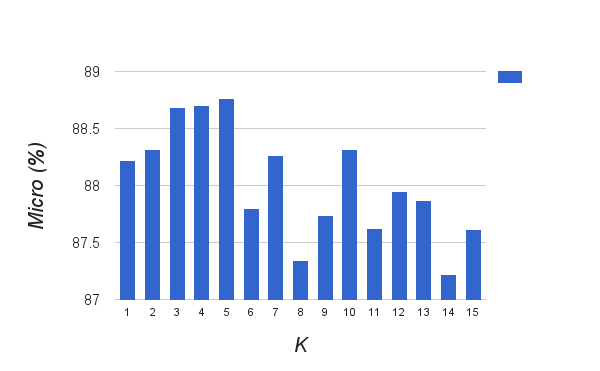
\includegraphics[width=\linewidth]{./k_effect.png}
\caption{Effect of parameter $K$ on entity linking accuracy.
Trained on CoNLL train and tested on CoNLL test-a.}
\label{fig:k_effect}
\end{figure}
}
% PGF plot version of the figure
{
\pgfplotsset{every tick label/.append style={font=\tiny}}
\begin{figure}[t!]
\centering
\resizebox {\columnwidth} {!} {
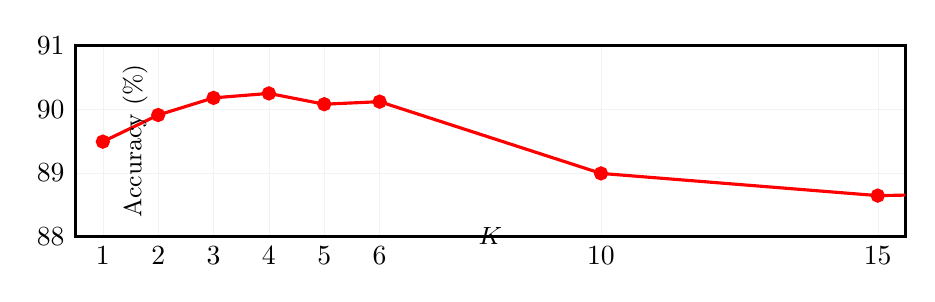
\begin{tikzpicture}
  \begin{axis}[
   %title  = Effect of K,
   width = \columnwidth,
   height=4cm,
%    ybar,
 %   bar width = 0.2cm,
    %x axis line style = { opacity = 0 },
    %axis y line       = none,
    tickwidth         = 0pt,
    xmin=0.5,xmax=15.5,
    ymin=88,ymax=91,
    grid=both,
    grid style={line width=.1pt, draw=gray!10},
    x label style={at={(axis description cs:0.5,0.1)},anchor=north},
    y label style={at={(axis description cs:0.1,.5)},anchor=south},
    xlabel={\small $K$},
    ylabel={\small Accuracy (\%)},
    mark size=2.0pt,
    line width=1.0pt,
   % enlarge y limits  = 0.2,
    xtick = data,
  ]
  \addplot [line width=0.4mm, red, mark=*, mark options=solid] coordinates { 
    (1,89.49) (2,89.91)  (3,90.18) (4,90.25) (5,90.08) (6,90.12) (10,88.99) (15,88.64) (20,88.72)
  };
  \pgfresetboundingbox
  %\addplot coordinates { (20,1)         (15,2)
   %                      (60,3)   (75,4)  };
 % \legend{Topics, Posts}
  \end{axis}
\end{tikzpicture}
}
\caption{Effect of parameter $K$ on entity linking accuracy.
Trained on CoNLL train and tested on CoNLL test-a. \label{fig:k_effect}}
\end{figure}
}

%(1,89.72) (2, 89.77) (3, 90.39) (4, 90.39) (5, 90.52)   (6,90) (7,90) (8,90) (9,90) (10,90)   (11,90) (12,90) (13,90) (14,90) (15,90)};


\subsection{Examples of gains (and losses)}


%
%\section{Conclusion}
%\label{sec:End}
%
%We have described two new approaches to modeling coherence for entity
%resolution.  While most existing systems consider all relations
%between entity candidates for a document to assign a coherence score
%to a candidate, we use a novel attention mechanism to select the most
%relevant relations.  Our experimental results support \hl{do they?}
%the premise that the inclusion of all relations can hurt performance.
%Our models improve the performance of a baseline system on three
%evaluation benchmarks, and our best multi-focal attention model
%achieves state-of-the-art results on standard benchmarks against
%highly competitive recently built systems.



%%% Local Variables: ***
%%% mode:latex ***
%%% TeX-master: "main.tex"  ***
%%% tex-main-file: "main.tex"  ***
%%% End: ***
